\section {СПЕЦИАЛЬНЫЙ РАЗДЕЛ}
В настоящем разделе будут описаны выбранный принцип реализации сбора логов из образцов и построенное для этого окружение. В нём будут использованы ссылки на скрипты ЯП Python (оканчиваются на .py), которые находятся в репозитории https://github.com/Vesemir/FinalProject/  в указанном относительно корня месте и реализуют описываемый функционал.

Поскольку хранение и обработку логов нельзя осуществлять на той же ОС, где будут исполняться вирусные образцы, данная деятельность будет осуществляться на специально сконфигурированной для этого ОС - "агенте". Существует два варианта организации работы схемы:
\begin {enumerate}
	\item Используя реальные ПК
	\item Используя виртуальные машины
\end {enumerate}
У варианта с реальным ПК есть свои преимущества, например, исчезает необходимость скрывать исполнение
образца в виртуальной машине, однако такой подход требует дополнительного ПК, и в случае,
если число агентов/ элементов окружения будет необходимо увеличить, нескольких. Восстановление агента
до изначального состояния может быть осуществлено с использованием специализированного ПО (FOG, fogproject.org).

В случае с виртуальными машинами, одного ПК будет достаточно. Однако, во-первых, это потребует дополнительных ресурсов самого ПК, во-вторых, существует множество техник для обнаружения исполнения кода в виртуальной среде, как специфичных для гипервизора, так и общих. Набор примерных техник обнаружения описан в  книге \cite{MALWAREANALYSIS} и может заключаться как в поиске присутствия конкретных имён процессов или ключей реестра, так и простом сканировании памяти на наличие строк "VMWare".  Как описано в статье \cite {VMMYTHS}, создатели гипервизоров разрабатывают ПО таким образом, чтобы уменьшить нагрузку,  необходимую для запуска ОС в виртуальной среде, следовательно, различия в поведении некоторых машинных инструкций в виртуальной среде и в реальной является следствием таковых упрощений реализации (например, VMWare эмулирует чипсет Intel 440BX для всех типов виртуальных машин, поскольку эмуляция всё появляющихся моделей и совместимого с ними оборудования потребовала бы слишком больших затрат и не принесла бы никакой практической с точки зрения производительности пользы). Для проверки возможных способов обнаружения виртуальной машины можно воспользоваться pafish (https://github.com/a0rtega/pafish). Однако, не следует считать наличие таких техник огромным недостатком использования виртуальных машин, т.к. в настоящее время вследствие простоты развёртывания и восстановления использование виртуальной инфраструктуры набирает популярность не только в целях исследования вирусов, но и в обычных организациях. Дальнейшее присутствие таких техник во вредоносном ПО и отказ от исполнения вредоносных действий в случае обнаружения будет наносить вред только лицам, его создающим.

Даже учитывая вышеупомянутые минусы виртуальных машин, всё же, возможность восстановления их до чистого состояния путём использования снапшотов представляется слишком удобной, чтобы обходиться без неё (гипервизор хранит на жёстком диске реального ПК разницу виртуальной оперативной памяти и разницу в секторах виртуального жёсткого диска в виде файлов, и просто восстанавливает файлы до исходного состояния). В качестве виртуальной среды была выбрана Oracle VirtualBox, поддерживающая снапшоты в бесплатной версии по сравнению с аналогичной продукцией от VmWare. Также, используется API VirtualBox для передачи файлов через предоставляемый Oracle модуль-обёртку на Python vboxapi (однако, факт использования данной реализации может быть использован в качестве одной из вышеупомянутых специфичных для VirtualBox техник обнаружения виртуальной машины, т.к. требует установки служб VirtualBox guest additions на агента, и поэтому возможно изменение подхода в дальнейшем). Помимо агента с ОС Windows, на котором будут исполняться исследуемые образцы, также используется виртуальная машина под управлением Debian 8 с установленным на неё пакетом INetSim, который предназначен для эмуляции многих сетевых служб. Поддерживая http, https, ftp, pop3 и многие другие протоколы, INetSim в том числе в состоянии по URL получаемого запроса определять тип файла и посылать в ответ поддельный файл такого же типа (.jpg, .ico, .exe и т.д.). Виртуальная машина с Debian помещается в ту же локальную сеть, что и  исследуемый агент, она же настраивается как сетевой шлюз для него, и одновременно - DNS сервер. Таким образом, на все поддерживаемые INetSim запросы, отправляемые с исследуемого агента на произвольные адреса, будет получен поддельный ответ, что должно позволить собрать больше информации о действиях образцов (например, скачивание и запуск исследуемым образцом поддельного .exe файла от INetSim свидетельствует о поведении, характерном для вредоносного ПО в основном служащего лишь каналом для загрузки другого вредоносного ПО).

По аналогии с последовательностью, описанной в статье \cite {MASSMALWARE}, получена следующая последовательность шагов, представляющая собой цикл исполнения образцов в VirtualBox. Их реализация находится в /vbox/tools/vmrun\_cycled.py

\begin {itemize}
	\item Предварительная конфигурация агента
	\item Загрузка образца
	\item Запуск отслеживающих инструментов и исполнение образца
	\item Получение логов
\end {itemize}

Для ускорения сбора представляется возможным параллельный запуск многих агентов Windows. При этом для каждого из них выполняется указанная последовательность шагов. Фактор ускорения сбора приблизительно равен числу используемых виртуальных машин с Windows. Выделив под основной ПК Intel Xeon e1245v3 (4-core, HyperThreading) и 10 Гб ОЗУ (отдельно для виртуальных машин) удалось добиться комфортной работы параллельно порядка 8--10 агентов Windows. Порядок взаимодействия виртуальных машин при использовании двух агентов Windows и основного ПК приведен на рис. \ref {fig:vmcycle}. При использовании большего числа агентов Windows порядок взаимодействия аналогичен, а ограничения на число агентов зависит в основном только от используемого аппаратного обеспечения.
\begin {figure}[H]
	\centering
	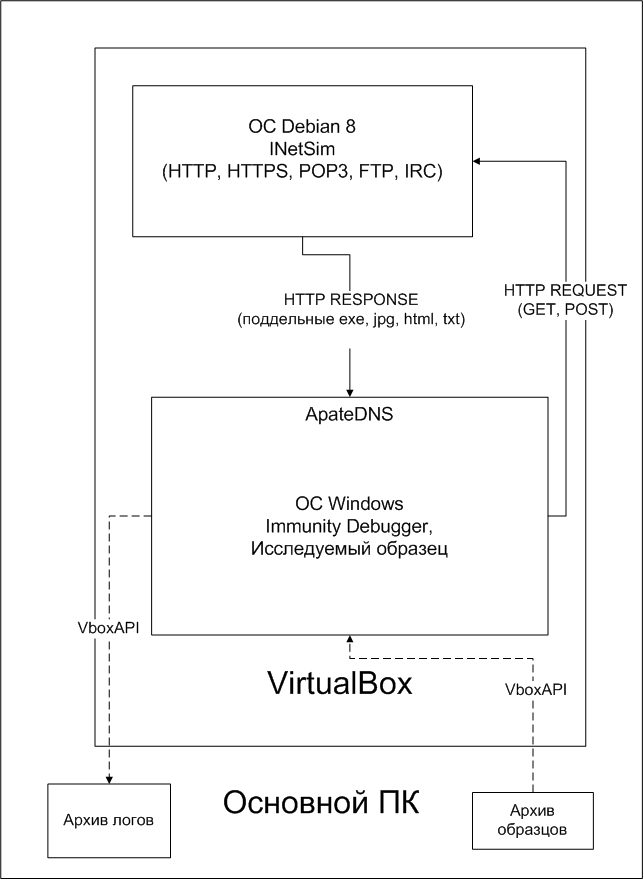
\includegraphics[width=\linewidth] {img/vmcycle.png}
	\caption {Порядок взаимодействия компонентов системы сбора логов}
	\label {fig:vmcycle}
\end {figure}

\subsection {Предварительная конфигурация  агента сбора логов}
\subsubsection {Настройка окружения}
Здесь большинство действий было выполнено однократно, после чего был создан снапшот состояния с настроенным окружением, готовым к запуску. Установлен отладчик Immunity Debugger, изменены его настройки, установлен Python 2.7.1, необходимый для работы отладчика, ApateDNS (утилита, позволяющая перенаправлять все DNS запросы на указанный IP адрес), .Net Framework 4.0, 4.5 (некоторые образцы основаны на данной платформе, и иначе запустить их не удастся), выключен файрвол Windows и служба контроля учётных записей (User account control).
Далее на этом шаге просто происходит возврат в "чистое состояние" исследуемого агента и виртуальной машины с INetSim.
\subsubsection {Маскировка виртуальной среды}
Для маскировки исполнения в виртуальной среде были применены следующие модификации виртуальной машины:
\begin {itemize}
	\item Добавлена информация из DMI (Desktop Management Interface)

	DMI позволяет программному обеспечению получать информацию из BIOS, об оборудовании и материнской плате (скопирована с основного ПК с использованием утилиты dmidecode).
	\item Добавлена таблица ACPI (Advanced Configuration and Power Interface)

	ACPI реализует интерфейс для управления питанием и конфигурации материнской платы и устройств. Для этого в оперативной памяти размещается несколько таблиц, содержащих методы управления ими и их описание. При помощи утилиты acpidump с основного ПК была скопирована такая таблица и подключена к виртуальной машине.
	\item Сгенерирован случайный MAC сетевой карты

	По умолчанию присваиваемые MAC адреса относятся к диапазону, начинающемуся с 08-00-27 и могут быть таким образом обнаружены. Вместо него взят случайный адрес из диапазона Intel.
	\item Изменена информация об HDD
	\item Изменена информация о CD-приводе
	\item Модифицированы разделы реестра

	Изменены разделы реестра SystemBiosDate, VideoBiosVersion и др., имеющие значение по умолчанию при создании виртуальной машины, позволяющие идентифицировать её как экземпляр VirtualBox.
\end {itemize}
Данный функционал реализуется в рамках vbox/tools/HideVBox/camouflage.py

\subsection {Загрузка исследуемого образца в агента}
VirtualBox предоставляет доступ к управлению различными функциями виртуальных машин через модуль-обёртку на ЯП Python, названную vboxapi. Используя его, реализован скрипт, скачивающий с основного ПК образец и скрипты, управляющие сбором логов.
\subsection {Запуск отслеживающих инструментов и исполнение исследуемого образца}
Поскольку снапшоты восстанавливаются из готового состояния, ApateDNS уже запущена и настроена на сервер INetSim.

Образец исполняется в отладчике, после чего специальный скрипт собирает информацию о присутствующих в таблице импортов исполняемого файла функций и устанавливает на них точки останова. Тот же скрипт регистрирует хук, в котором описаны необходимые для получения параметры в случае вызова таковых функций.
В случае вызова функции, отладчик логирует всё в файл. Образец исполняется в течение двух минут.
\subsection {Сбор полученных данных}
По истечении указанного промежутка времени скрипт через vboxapi забирает собранные логи о деятельности образца и выключает обе виртуальные машины. После этого происходит выборка из архива следующего образца и запуск следующей итерации цикла для его исследования.

\subsection {Требования к алгоритму сравнения цепочек}
 Для принятия решения о нахождении похожих цепочек вызовов в логах необходимо выбрать способ. Далее будет описан выбранный алгоритм, позволяющий находить не только идентичные цепочки, но и видоизменённые до определённой степени вставленными в них дополнительными вызовами, например:

kernel32.OpenFile -> kernel32.SetFilePointer -> kernel32.Sleep -> kernel32.WriteFile

vs

kernel32.CreateFile -> kernel32.SetFilePointer -> ---  ->   kernel32.WriteFile

Указанные цепочки будут совмещены как похожие, если в матрице цен указать достаточное значение близости OpenFile к CreateFile.
В данном случае пропуск  вызова (символа) при сравнении двух последовательностей будет обозначаться как ``---'', и аналогичен совмещению (kernel32.Sleep, --- ) при выравнивании цепочек.
\subsection {Приведение собранных данных к удобной для обработки форме}
Собранные текстовые логи работы вредоносных образцов являются достаточно информативными с точки зрения ручного анализа, однако для автоматической обработки их следует привести к более компактной и быстрее обрабатываемой форме (как правило, в любых языках программирования операции над строками медленнее операций над числовыми данными). Для анализа цепочек было решено хранить информацию о вызовах как массив из int32 (4 байта на один вызов). Такая форма достаточна для хранения более чем 4 миллионов различных вызовов, а также она поддерживается пакетом numpy ЯП Python. При этом словарь, отображающий эти числа обратно в фактические имена (и, возможно, параметры) функций хранится отдельно. Это позволяет в дальнейшем возвращать более подробную информацию о найденных совпадениях цепочек.

Поскольку размер цепочек произволен, хранение в отдельном файле каждой цепочки потенциально может привести к напрасной трате места хранения на жёстком диске. Например, цепочка длиной в 100 вызовов, занимающая согласно выбранной форме представления 400 байт, будет фактически иметь минимальный размер файла величиной с установленный кластер (обычно 4096 байт). Поэтому для хранения массивов numpy был выбран формат HDF5 (Hierarhical Data Format, иерархический формат данных). Он поддерживает хранение в одном файле некоторого подобия иерархической файловой системы, состоящей из массивов numpy, при этом к каждой отдельной цепочке может быть получен доступ по уникальному имени пути. Это позволяет решить проблему затрат лишнего места на хранение, т.к. теперь как максимум будет потеряно до 4  килобайт на все цепочки целиком. Для работы с файлами такого формата в ЯП Python присутствует модуль h5py.
 Реализация данного преобразования хранится в /lib/pander.py.
\subsection {Реализация алгоритма нахождения оптимального локального выравнивания}
Для сравнения как бинарных, так и текстовых строк (или в нашем случае --- последовательности чисел) классической метрикой является расстояние Левенштейна (также называемое дистанцией редактирования). Между двумя строками дистанцией редактирования будет являться число базовых операций, применяемых к одной строке, чтобы получить другую. К базовым операциям относятся:
\begin {itemize}
	\item Вставка одного символа
	\item Удаление одного символа
	\item Замена одного символа на другой
\end {itemize}
Эта  метрика используется в алгоритме Смита-Ватермана, впервые опубликованном в \cite{LOCALALIGNMENT}. Несмотря на то, что придуман он был для нахождения участков похожих цепочек нуклеотидных последовательностей и относится к генетике, можно упомянуть, что некоторые авторы \cite{BLACKBOOK} относятся к проблеме компьютерных вирусов как к искусственной форме жизни (если точнее, то self-replicating automata, "самовоспроизводящийся автоматический механизм"), поэтому идеи ближе, чем может показаться на первый взгляд.

Существует два основных подхода к сравнению последовательностей: глобальное и локальное выравнивание. Применение глобального выравнивания требует примерно одинаковой длины цепочек, что нельзя гарантировать в случае исследования произвольных образцов. Использование глобального выравнивания можно было бы отнести к поиску практически идентичных копий вредоносных образцов. Алгоритм Смита-Ватермана применяет локальное выравнивание, что ближе к идее нахождения каких-либо распространённых сходных отрезков последовательностей вызовов функций API, потенциально обладающих вредоносным воздействием. Он берёт две последовательности произвольной длины и находит оптимальное выравнивание в любом месте последовательности согласно задаваемой матрице цен, определяющей изменение счёта текущего выравнивания. 

Набор шагов алгоритма для строк $A = a_1 a_2 a_3 ... a_n$ , $B = b_1 b_2 b_3 ... b_m$ длины n и m соответственно заключается в следующем:
\begin {enumerate}
	\item Вычисляем матрицу выравниваний

	Двумерная матрица размерностью n на m инициализируется нулями. В случае использования локального выравнивания первый столбец и первая строка остаются равными 0, чтобы позволить новому выравниванию начаться в любом месте строки без штрафа за вставку первоначальных символов, идущих до выравнивания. Далее матрица продолжает заполняться слева направо и сверху вниз, при этом каждое новое значение выбирается как максимальное из трёх вариантов:
	\begin {itemize}
		\item Цена совмещения очередного символа первой и второй строки $(a_i, b_j)$ плюс цена, стоящая в матрице выравнивания сверху слева по диагонали (предыдущая цена совмещения двух предыдущих символов строк).
		\item Цена вставки символа первой строки (аналогична совмещению $(a_i, -)$), при этом т.к. не произошло продвижения по символам второй строки, добавляется цена из ячейки, находящаяся сверху от текущей.
		\item Цена вставки символа второй строки (аналогична совмещению $(-, b_j)$), при этом т.к. не произошло продвижения по символам первой строки, добавляется цена, расположенная в матрице слева от вычисляемой ячейки.
	\end {itemize}
	Если получаемое при выборе максимума число отрицательное, вместо него записывается 0, чтобы данная ячейка массива не влияла на нахождение возможных последующих локальных выравниваний.
	После завершения операций матрица выравниваний готова.
	\item Вычисление локального выравнивания

	Задача заключается в обходе матрицы выравниваний по определённым правилам:
	\begin {itemize}
		\item На первом шаге находится максимальное значение цены в матрице и запоминаются индексы позиции (i, j), на которой он располагается
		\item Далее с позицией максимума сравниваются ячейки, стоящие выше, слева и по диагонали от неё, чтобы понять, каким из 3х путей этой ячейке было присвоено значение, соответственно производится уменьшение индекса i, j или обоих сразу, реконструируется часть строки выравнивания, после чего операция повторяется
		\item В случае, если значение ячейки, на которую указывают текущие значения индексов (i, j) равно 0, алгоритм завершает работу, возвращая пару реконструированных строк и счёт оптимального выравнивания
	\end {itemize}
	При необходимости алгоритм можно модифицировать для нахождения нескольких пар выравниваний со значениями меньше, чем у оптимального.
\end {enumerate}

В текущей реализации матрица весов модифицирована следующим образом: вручную указан набор функций, обладающих малой информативностью и при их совмещении добавляется цена 0, также был выбран определённый набор критичных функций, для которых оценка при совпадении вызовов несколько выше, чем для остальных. Для лучшей точности работы следует выдавать близкие оценки функциям, имеющим сходные наборы аргументов и/ или близких по реализуемому ими функционалу (по крайней мере, ASCII/Unicode версиям функций плюс их обычным и Ex вариантам).

Наибольшую трудоёмкость данного алгоритма составляет шаг построения матрицы выравниваний. Если считать, что в среднем длина двух сравниваемых цепочек одинакова, и приняв за n длину цепочки, асимптотическая оценка функции роста трудоёмкости данного алгоритма составляет $O(n^2)$. В связи с этим, было принято решение ускорить реализацию данного шага. Это было произведено в рамках использования Cython. Cython - отдельный диалект ЯП Python, позволяющий получить значительное ускорение выполнения трудоёмкого кода через создание расширения, которое будет преобразовано к ЯП C и скомпилировано.  Значительного прироста скорости исполнения можно добиться, всего лишь статически типизировав переменные. После компиляции данное расширение может быть импортировано в обычный Python и использовано без каких-либо дополнительных ограничений. Cython-расширение реализовано в рамках /lib/seq\_analyzer/scoring/compare\_samples.pyx.

После применения преобразования в файл hdf5 логов и сохранения полученный набор последовательностей может  быть в любой момент вновь пропущен через алгоритм на новых образцах. 
Алгоритм локального выравнивания реализован в /lib/seq\_analyzer/local\_alignment.py

В итоге, для предоставления возможности запуска исследования образца, преобразования логов к используемой в настоящей работе форме, а также осуществления выравнивания полученных цепочек была реализована утилита командной строки cli-launcher.py, позволяющая вызывать данный функционал как по отдельности, так и полной последовательностью преобразований. Далее для удобства развёртывания на новых ПК данная утилита была упакована с помощью программы PyInstaller, позволяющей из скриптов ЯП Python создавать исполняемые файлы формата, используемого ОС. Описание реализуемого функционала и предлагаемые для использования опции доступны передачей аргумента -h в данную утилиту.
\subsection {Выводы по разделу}
В рамках настоящего раздела была сконструирована и реализована схема исполнения исследуемых образцов в целях сбора цепочек вызовов и выбран способ компактного хранения этих данных, допускающий последующую многократную и быструю обработку.

Также был найден алгоритм, позволяющий находить близкие цепочки вызовов в собранных данных согласно поставленным для программного модуля целям и проведена его программная реализация, а также оптимизация скорости исполнения.

Результат реализации и управление программным модулем доступны через утилиту командной строки cli-launcher.